%\documentclass[11pt, oneside]{article}  
%\lfoot{Enzia Schnyder} %your name in the footer

% Note: Packages are already included at the top in global_handouts.tex
%\usepackage{style-3yp} %this is the .sty file
%\usepackage{pdflscape}
%\usepackage{float}
%\usepackage{longtable}
%table
%\usepackage{array}
%\newcolumntype{L}{>{\centering\arraybackslash}m{2.5cm}}
%\newcolumntype{J}{>{\centering\arraybackslash}m{4.1cm}}
%\newcolumntype{M}{>{\centering\arraybackslash}m{5cm}}
%\newcolumntype{N}{>{\centering\arraybackslash}m{3.5cm}}
%\usepackage{multirow}
%\usepackage{gensymb} %degrees symbol
%\usepackage [version=4] {mhchem}

%\begin{document}
\section{Gas Turbine}

\begin{table} [h]
\begin{center}
\caption{Properties of the ammonia-air mixture. Lower and upper flammability limits (LFL \& UFL) are measured by volume percentage of air [Slide 43]} \label{tab:mixproperties}
\begin{tabular}{ |c|c|c|c|c|c| }
 \hline
& Mr (a.m.u) & LCV (MJ/kg) \cite{website:spg}& LCV (MJ/kmol) & LFL (\%)& UFL (\%) \\ 
 \hline
  $H_2$ & 2.02 & 120.1 & 242.6 & 4.0 & 75.0\\ 
 \hline
$NH_3$ & 17.03 & 18.6 & 316.8 & 15.0 & 28.0\\ 
 \hline
$H_2/NH_3$ mixture & 10 & 28.6 & 281.3 & 6.47 & 40\\
 \hline
\end{tabular}
\end{center} 
\end{table}

%\begin{equation}
%\ce{(0.62 NH_3 + 0.19 N_2 + 0.57 H_2) + 0.75\lambda(O_2 + 3.76 N_2^*) ->1.5H_2O + 0.5N_2 + 2.82\lambda N_2^* + 0.75(\lambda \ \hyphen \ $1$ )O_2}
%\end{equation}

\begin{figure} [h]
\centering
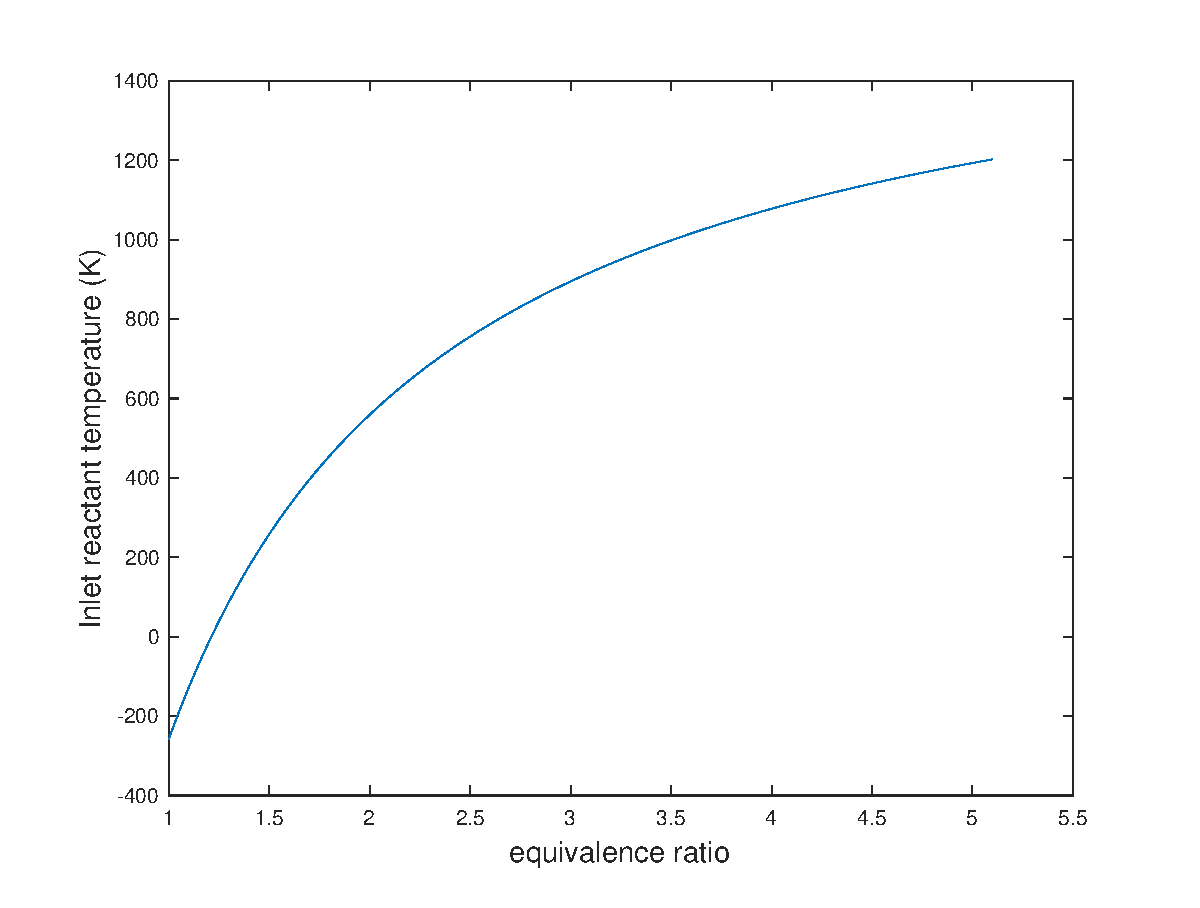
\includegraphics[width=0.65\textwidth]{./pictures/combustor.eps}
  \caption{Variation in inlet reactant temperature with equivalence ratio. [Slide 44]} \label{fig:flametemp}
  \end{figure} 
\begin{figure} [H]
\centering
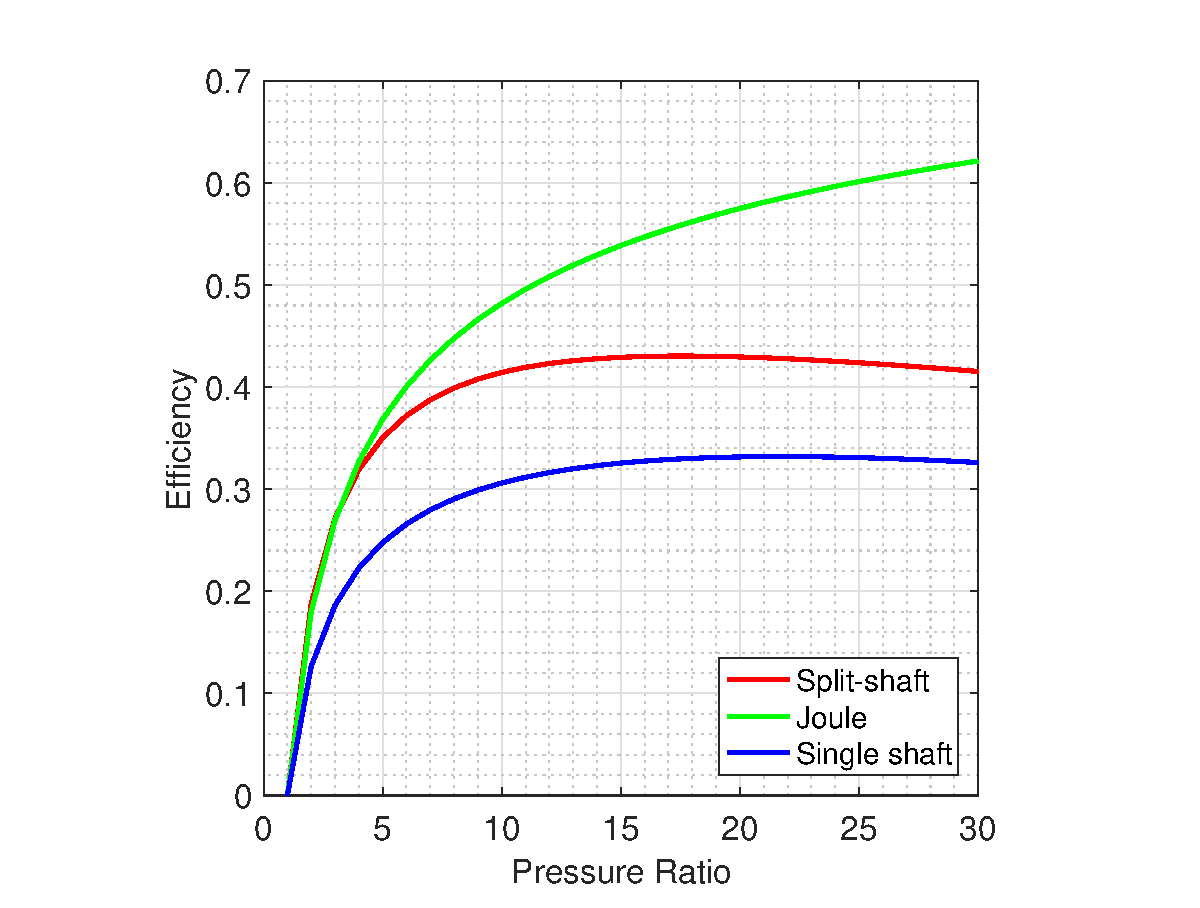
\includegraphics[width=0.65\textwidth]{./pictures/efficiencyPT.eps}
  \caption{Chart showing the change in joule efficiency, split-shaft efficiency and simple cycle efficiency across different pressure ratios [Slide 44]} \label{fig:twinefficiency}
  \end{figure}
  
\begin{figure} [H]
\centering
\includegraphics[width=0.58\textwidth]{./pictures/plantdiagram.png}
  \caption{The turbine diagram, showing all streams, work inputs, outputs and heat inputs [Slide 45]} \label{fig:turbinediagram}
  \end{figure}
  
  \begin{table} [h]
\begin{center}
\caption{Heat inputs and work outputs of the system [Not include in presentation slides]} \label{tab:powerdata}
\begin{tabular}{ |c|c| }
 \hline
  $W_{T1}$ & 82.6 MW\\ 
 \hline
  $W_{T2}$ & 89.3 MW\\
  \hline
  $W_E$ & 723.6 kW\\
 \hline
 $Q_{in}$ & 207 MW\\
 \hline
 Overall Efficiency & 0.4353\\ 
 \hline
\end{tabular}
\end{center}  
\end{table}

  \begin{table} [h]
\begin{center}
\caption{Initial and final properties of the each turbine at full load [Slide 45]} \label{tab:powerdata}
\begin{tabular}{ |c|c|c| }
 \hline
  Model & Initial & Final\\ 
 \hline
   NH3 flow rate (kmol/s) & 0.3246 & 0.6257\\
  \hline
  Equivalence ratio & 2.50 & 2.44\\
 \hline
  Efficiency & 0.3320 & 0.4353\\
 \hline
\end{tabular}
\end{center}  
\end{table}


\bibliography{handouts}
\bibliographystyle{unsrt}

%\end{document}
